\section{Evaluation}

In this section, we evaluate the performance of our implementation of the flattened page table in Linux. We first present the experimental setup, including the hardware and software configurations. Then, we compare the performance of our implementation with the original 4-level radix paging mechanism, and the ECPT paging mechanism in Linux using various benchmarks. Finally, we analyze the results and discuss the implications of our findings.

% TODO: add reference for ECPT, csynb

\subsection{Methodology and Metrics}

To evaluate the performance of our Flattened Page Table (FPT) implementation, we designed a comprehensive evaluation pipeline that executes benchmarks inside QEMU virtual machines, collects low-level memory traces, and performs offline analysis using instrumentation and custom tooling. Our methodology ensures consistency and fairness when comparing FPT against the baseline 4-level Radix Tree paging and the ECPT mechanism.

We run various benchmarks inside QEMU virtual machines with different configurations, including the original 4-level radix paging, the ECPT mechanism, and two configurations, L3L2 mode and L4L3+L2L1 mode, of our FPT implementation. The benchmarks include a mix of workloads that stress different aspects of the memory management system, such as memory allocation, page table lookups, and memory-intensive applications. For each benchmark, we split the execution into loading and running phases. The loading phase is used to load the benchmark into memory, while the running phase is used to execute the benchmark. We measure the execution time of each phase separately to understand the impact of our FPT implementation on both loading and running times.

During executing the benchmarks, we collect low-level memory traces using DynamoRIO, a dynamic binary instrumentation framework. We collect information about memory accesses, page walk latencies, TLB misses, instruction counts, and some other performance metrics. We then generate some visualization graphs to help partition the memory access of each execution of benchmarks and compare the performance of the different configurations.

\subsection{Benchmarks}

We selected a diverse set of benchmarks to evaluate the performance of our FPT implementation.

We use seven memory-intensive macro benchmarks. Some benchmarks are selected from the GraphBIG benchmark suite, which is a collection of graph processing workloads. The benchmarks include: 
    Breadth-First Search (BFS),
    Depth-First Search (DFS),
    Degree Centruality (DC),
    Single-Source Shortest Path (SSSP),
    Connected Components (CC),
    Triangle Counting (TC),
    PageRank (PR).

We also run the GUPS benchmark for random memory access, and a memory test from SysBench. Both benchmarks have 64GB working sets.

\begin{table}
    \centering
    \footnotesize
    \setlength{\tabcolsep}{2pt}
    \begin{tabular}{lcccc}
        \toprule
        \textbf{Application} & \textbf{Working Set} & {\bf \# Records} & \textbf{Read:Write} & {\bf \# Requests} \\
        \midrule
        Redis      & 128 GB & 536 M & 50:50 & 60 M \\
        Memcached  & 69 GB  & 56 M  & 80:20 &  10 M \\
        PostgreSQL & 64 GB  & 21 M & 100:0 & 25 M \\
        \bottomrule
    \end{tabular}
    \caption{\bf Application workloads used in the evaluation.}
    \label{table:workloads}
\end{table}

\begin{figure}
    \centering
    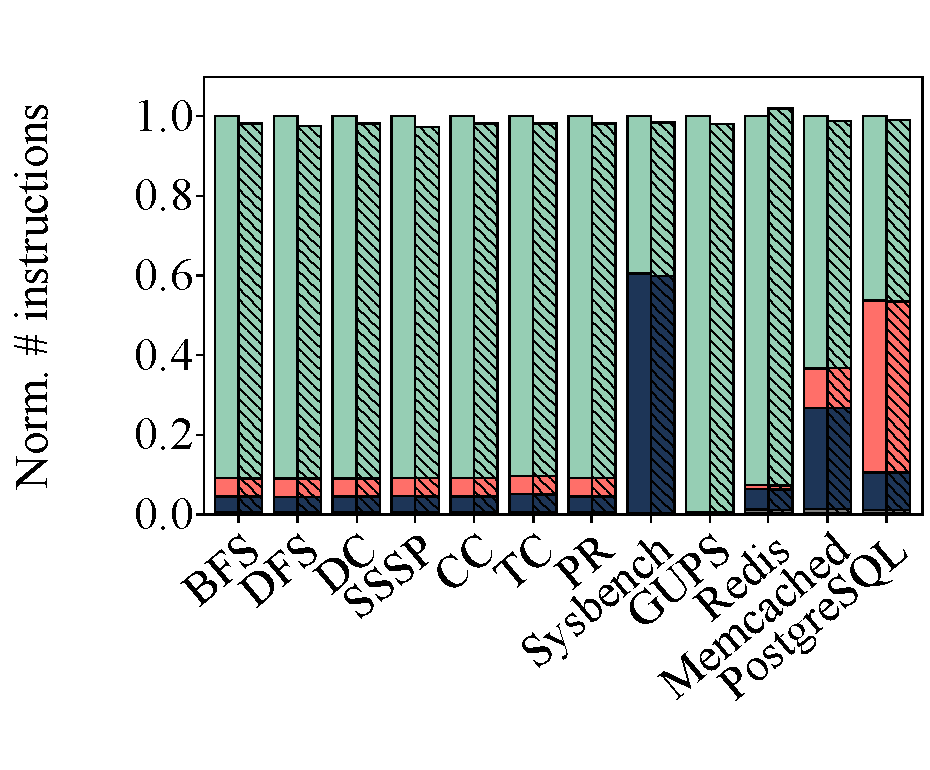
\includegraphics[width=0.495\linewidth]{graph/kern_inst_unified_never_L3L2.pdf} 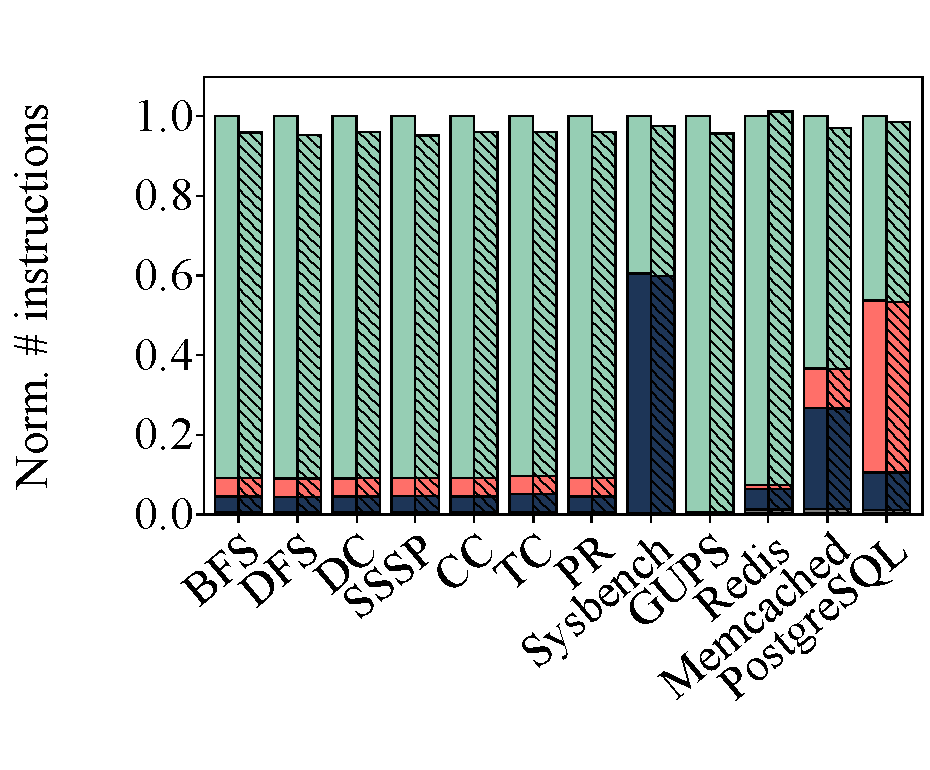
\includegraphics[width=0.495\linewidth]{graph/kern_inst_unified_never_L4L3L2L1.pdf}
    \caption{Distribution of kernel instructions of EMT-Linux with the Radix and FPT L3L2 mode (left) and L4L3+L2L1 mode (right).}
    \label{fig:kernel_inst}
\end{figure}

We also keep track of three memory-intensive real-world applications:
    Redis,
    Memcached,
    PostgreSQL.
Table \ref{table:workloads} summarizes the workloads of these applications.

% TODO: citation for GraphBIG

\subsection{Results}

\subsubsection{OS Overhead of FPT}

Figure~\ref{fig:kernel_inst} shows the distribution of kernel instructions under the Radix paging and two Flattened Page Table (FPT) configurations: L3L2 mode (left) and L4L3+L2L1 mode (right). The shaded areas represent instructions executed under FPT modes, while the blue, red, green, and gray segments correspond to instructions related to timers, system calls, page faults, and other kernel activities, respectively. Compared to the Radix baseline, both FPT modes show a slight reduction in the total number of kernel instructions, with a more noticeable decrease in the L4L3+L2L1 configuration.

We believe that the reduction in kernel instructions is primarily due to the decreased number of page table walks and TLB misses. The kernel instruction reduction in L4L3+L2L1 mode could be because the L4L3+L2L1 mode reduces one more page table level that need to be traversed during address translation, leading to fewer kernel instructions related to page table lookups. Overall, these results demonstrate that FPT, especially the more aggressive L4L3+L2L1 mode, can alleviate kernel instruction overhead and improve execution efficiency for memory-intensive applications.

\subsubsection{Performance Comparison}

\begin{figure}
    \centering
    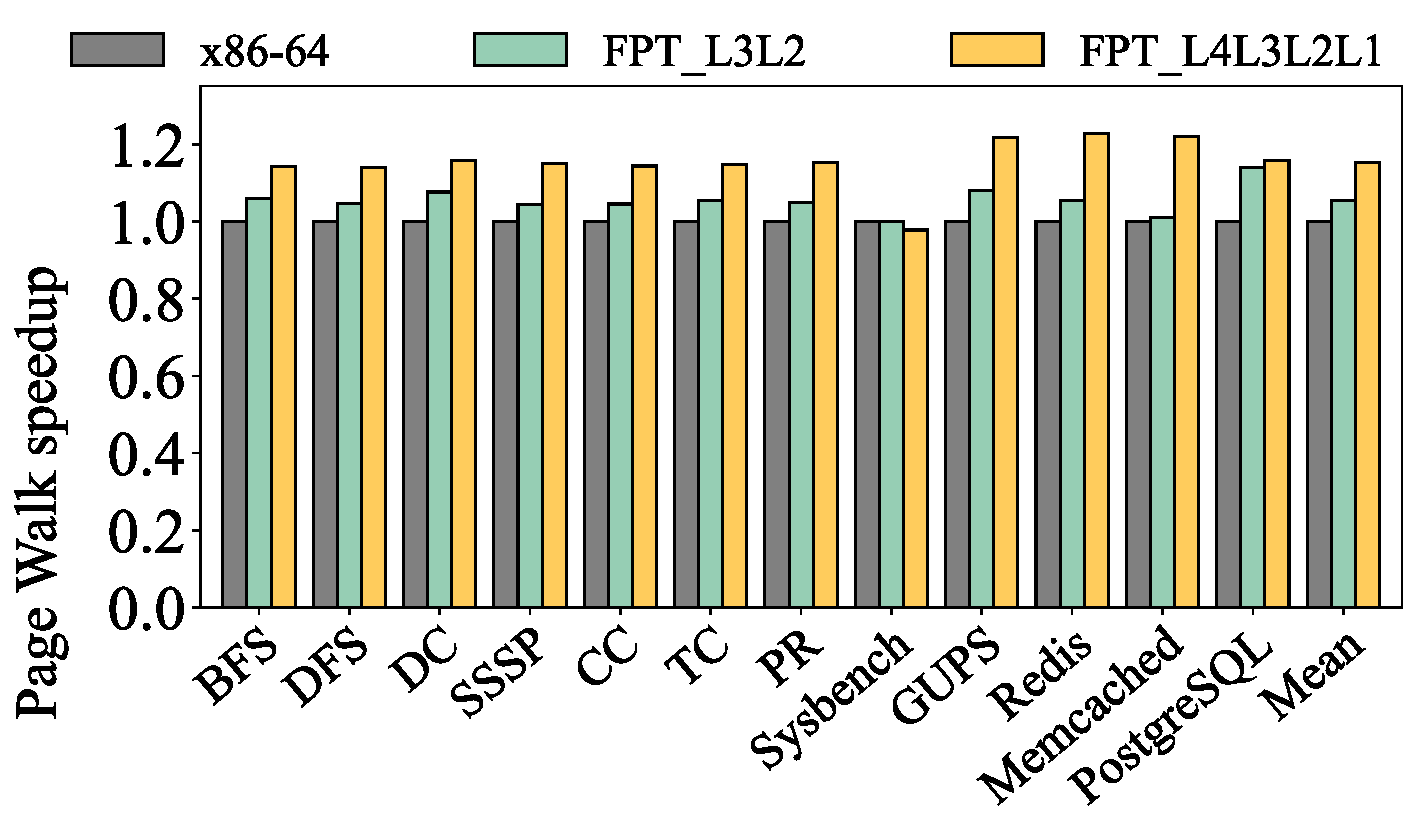
\includegraphics[width=0.85\linewidth]{graph/fpt_pgwalk_unified_never.pdf}
    \caption{Page Walk Latencies of Radix and FPT modes}
    \label{fig:fptpgwalk}
\end{figure}

\begin{figure}
    \centering
    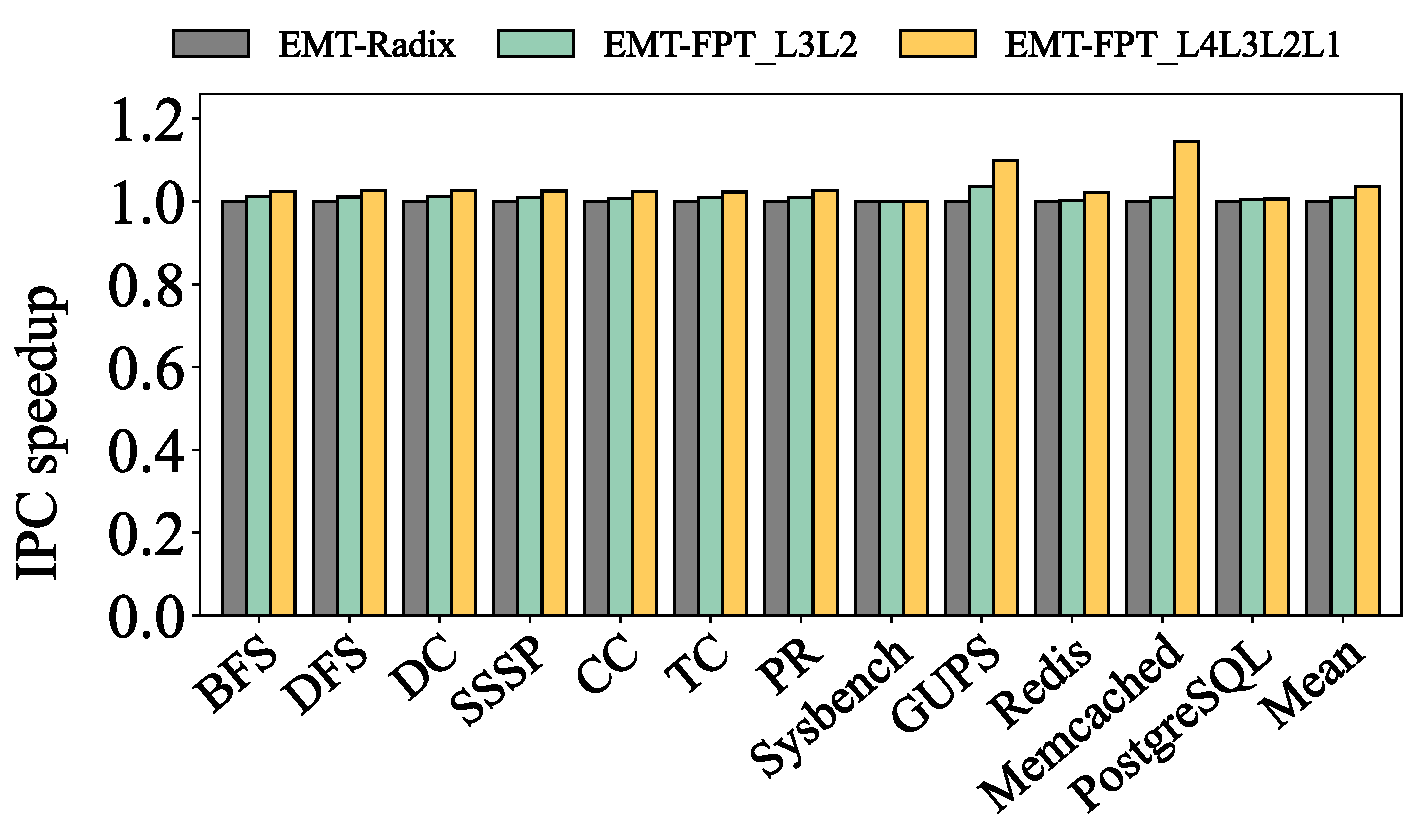
\includegraphics[width=0.85\linewidth]{graph/fpt_ipc_unified_never.pdf}
    \caption{IPC Speedup of Radix and FPT modes}
    \label{fig:fptipc}
\end{figure}

\begin{figure}
    \centering
    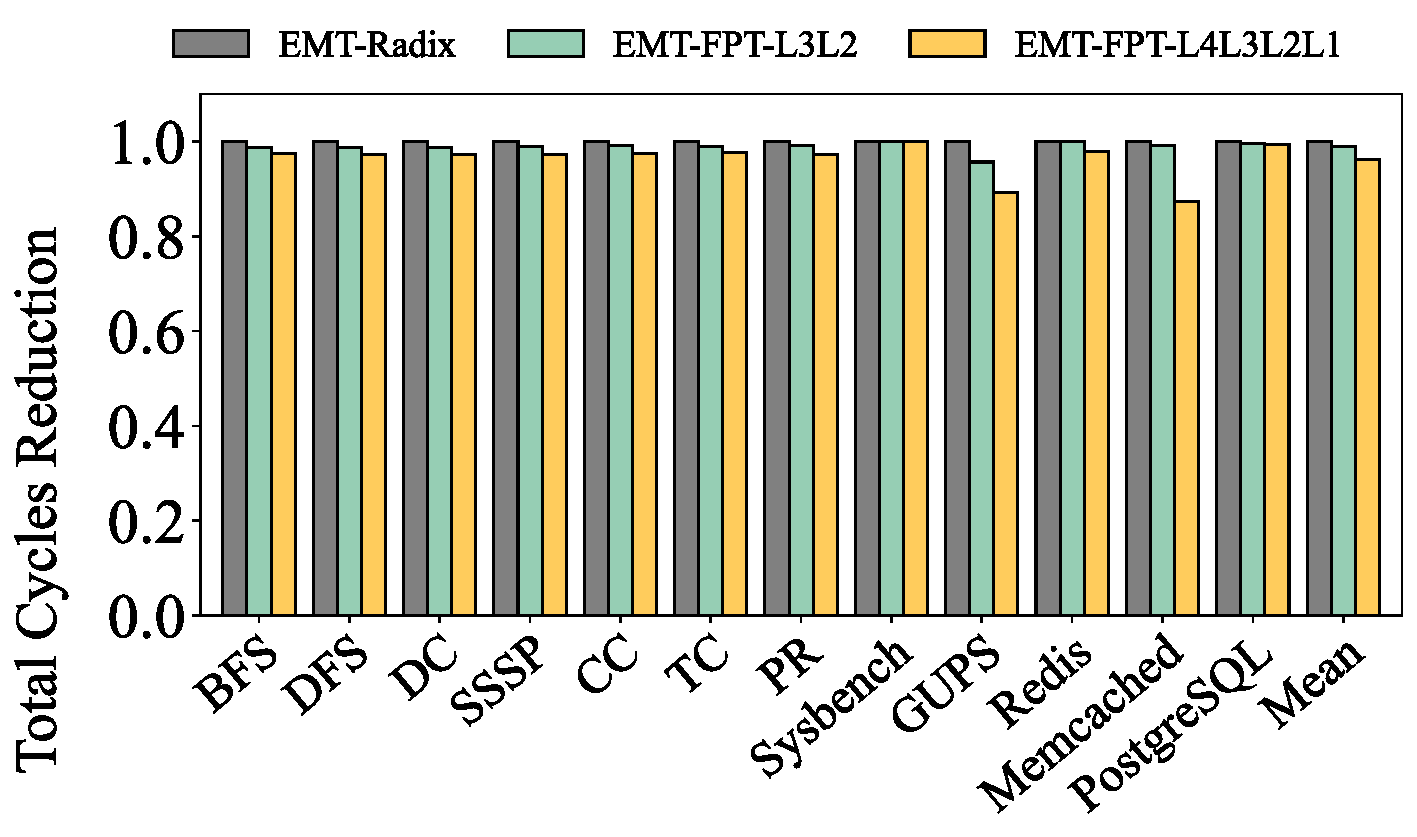
\includegraphics[width=0.85\linewidth]{graph/fpt_e2e_unified_never.pdf}
    \caption{End-to-End Latency of Radix and FPT modes}
    \label{fig:fpte2e}
\end{figure}

